\documentclass[border=6pt]{standalone}
% Shared typography and colours for the standalone figures.
\usepackage{unicode-math}
\setmainfont{TeX Gyre Heros}
\setmathfont{TeX Gyre Pagella Math}
\usepackage{tikz}
\usetikzlibrary{arrows.meta,positioning,calc,decorations.pathreplacing}
\usepackage{pgfplots}
\pgfplotsset{compat=1.18}

% One colour per element or subsystem. Record the mapping in
% the working repository conventions and use it identically in every figure.
\definecolor{elemA}{HTML}{1F5FA8}
\definecolor{elemB}{HTML}{B8461B}
\definecolor{elemC}{HTML}{2E7D32}
\definecolor{elemD}{HTML}{6A4C93}
\definecolor{frameline}{HTML}{555555}

\begin{document}
\hyphenpenalty=10000
\exhyphenpenalty=10000
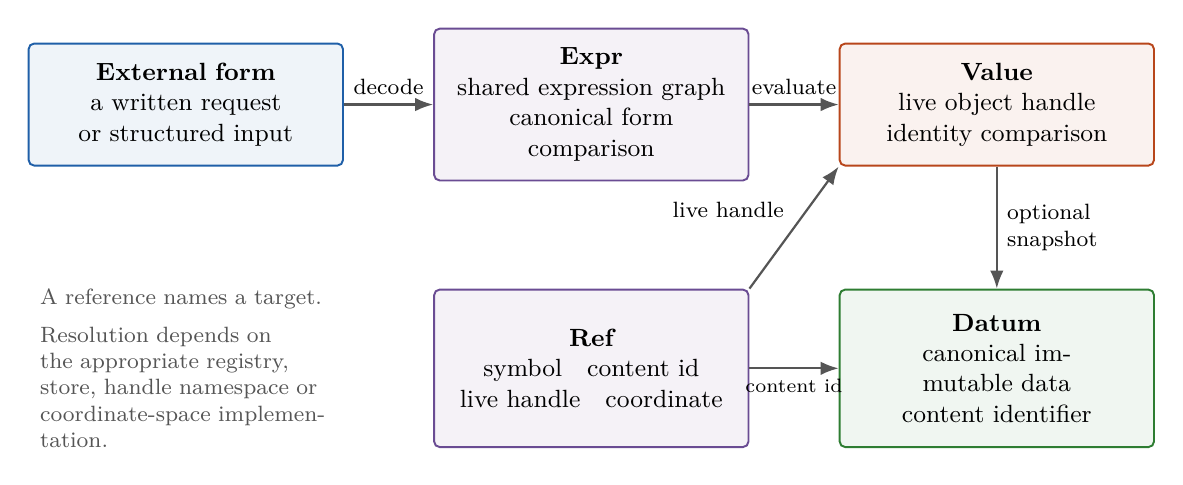
\begin{tikzpicture}[font=\small,
box/.style={draw=#1,fill=#1!7,rounded corners=2pt,line width=.7pt,text width=3.5cm,minimum height=1.55cm,align=center,inner sep=7pt},
arrow/.style={-{Latex[length=2.3mm]},line width=.8pt,draw=frameline}]
\node[box=elemA] (source) at (-5.15,3.1) {\textbf{External form}\\a written request\\or structured input};
\node[box=elemD] (expr) at (0,3.1) {\textbf{Expr}\\shared expression graph\\canonical form comparison};
\node[box=elemB] (value) at (5.15,3.1) {\textbf{Value}\\live object handle\\identity comparison};
\draw[arrow] (source)--node[above,font=\footnotesize]{decode}(expr);
\draw[arrow] (expr)--node[above,font=\footnotesize]{evaluate}(value);
\node[box=elemD,minimum height=2cm] (ref) at (0,-.25) {\textbf{Ref}\\symbol\quad content id\\live handle\quad coordinate};
\node[box=elemC,minimum height=2cm] (datum) at (5.15,-.25) {\textbf{Datum}\\canonical immutable data\\content identifier};
\draw[arrow] (value)--node[right,font=\footnotesize,align=left]{optional\\snapshot}(datum);
\draw[arrow] (ref.east)--node[below,font=\scriptsize]{content id}(datum.west);
\draw[arrow] (ref.north east)--node[above left,font=\footnotesize]{live handle}(value.south west);
\node[align=left,text width=3.7cm,font=\footnotesize,text=frameline] at (-5.15,-.25)
 {A reference names a target.\\[4pt] Resolution depends on the appropriate registry, store, handle namespace or coordinate-space implementation.};
\end{tikzpicture}
\end{document}
